% Created by tikzDevice version 0.12.6 on 2024-09-26 13:54:13
% !TEX encoding = UTF-8 Unicode
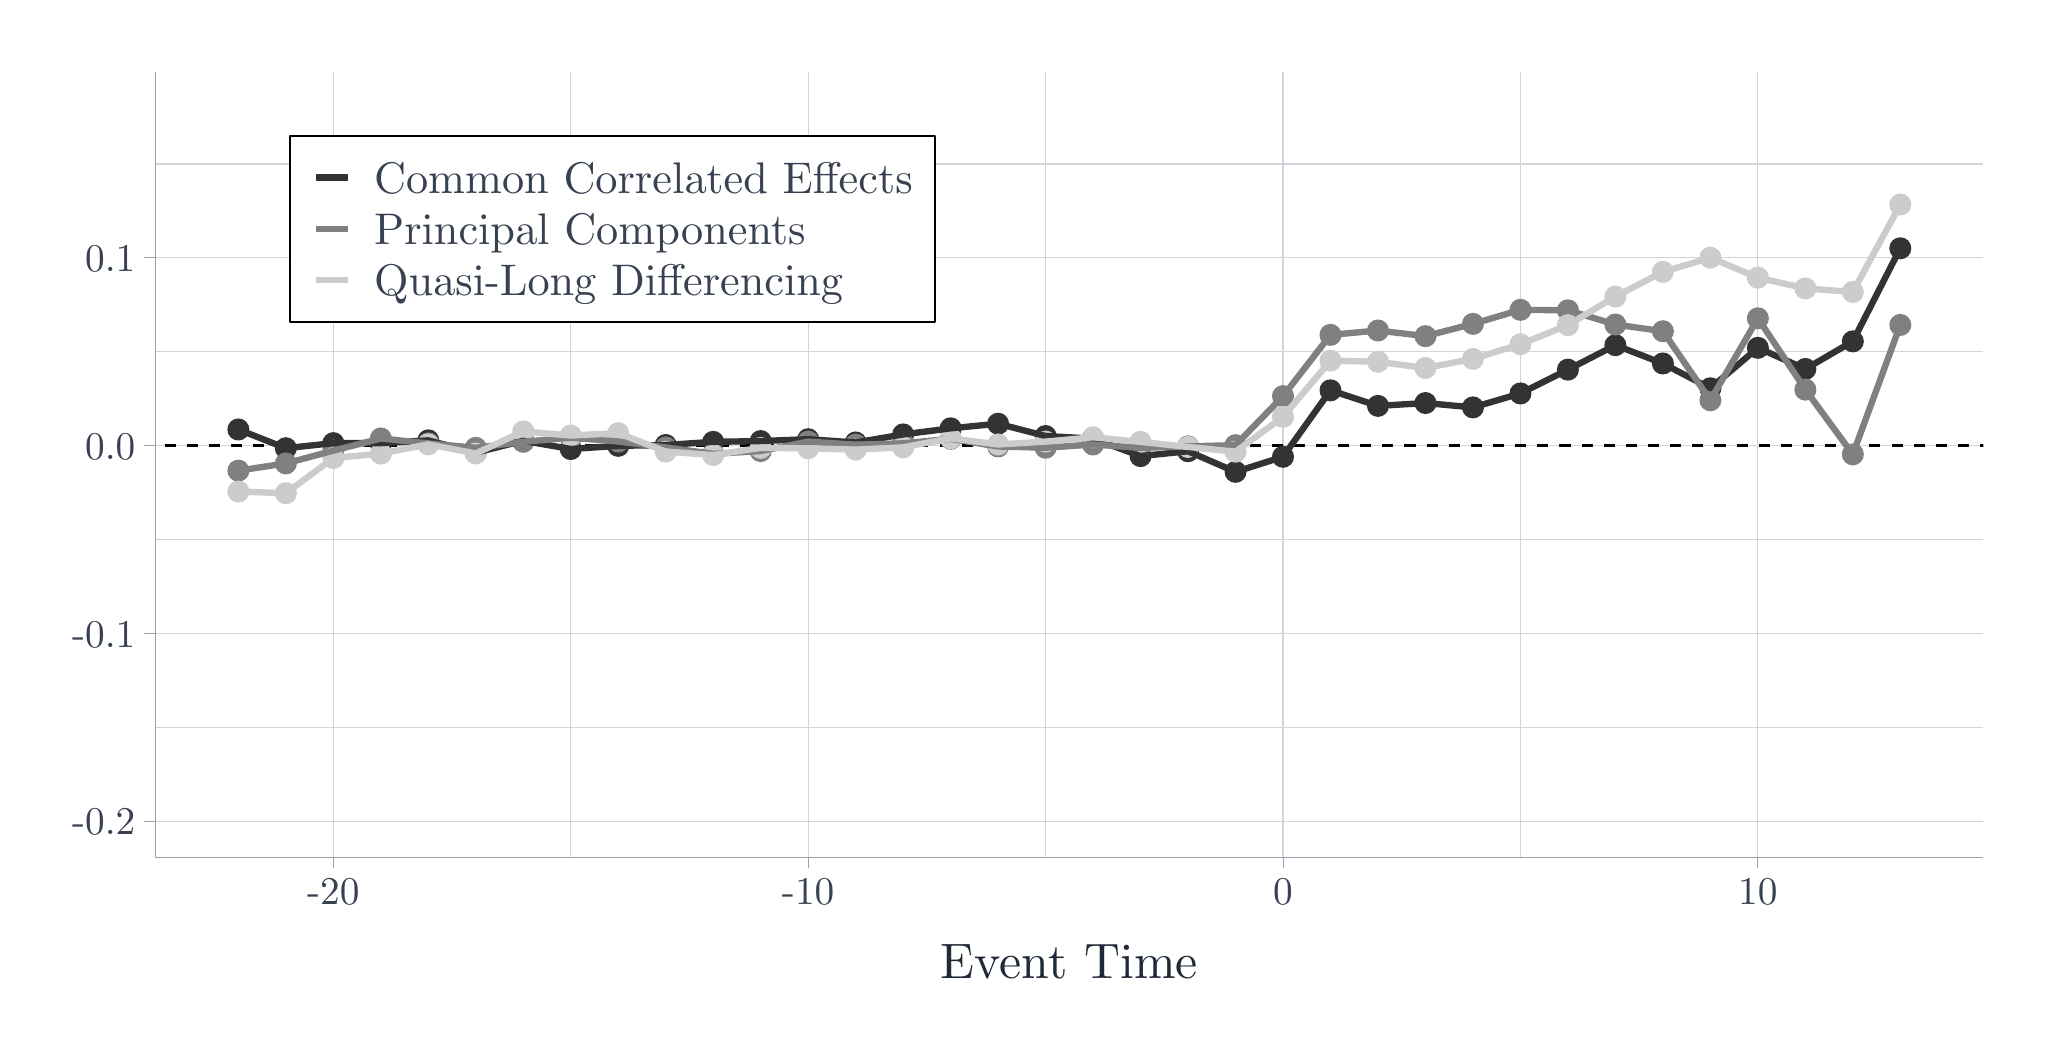
\begin{tikzpicture}[x=1pt,y=1pt]
\definecolor{fillColor}{RGB}{255,255,255}
\path[use as bounding box,fill=fillColor] (0,0) rectangle (722.70,361.35);
\begin{scope}
\path[clip] (  0.00,  0.00) rectangle (722.70,361.35);
\definecolor{drawColor}{RGB}{255,255,255}

\path[draw=drawColor,line width= 0.8pt,line join=round,line cap=round,fill=fillColor] (  0.00,  0.00) rectangle (722.70,361.35);
\end{scope}
\begin{scope}
\path[clip] ( 46.10, 61.65) rectangle (706.70,345.35);
\definecolor{drawColor}{RGB}{255,255,255}
\definecolor{fillColor}{RGB}{255,255,255}

\path[draw=drawColor,line width= 0.8pt,line join=round,line cap=round,fill=fillColor] ( 46.10, 61.65) rectangle (706.70,345.35);
\definecolor{drawColor}{RGB}{209,213,219}

\path[draw=drawColor,line width= 0.4pt,line join=round] ( 46.10,108.48) --
	(706.70,108.48);

\path[draw=drawColor,line width= 0.4pt,line join=round] ( 46.10,176.35) --
	(706.70,176.35);

\path[draw=drawColor,line width= 0.4pt,line join=round] ( 46.10,244.22) --
	(706.70,244.22);

\path[draw=drawColor,line width= 0.4pt,line join=round] ( 46.10,312.09) --
	(706.70,312.09);

\path[draw=drawColor,line width= 0.4pt,line join=round] (196.24, 61.65) --
	(196.24,345.35);

\path[draw=drawColor,line width= 0.4pt,line join=round] (367.82, 61.65) --
	(367.82,345.35);

\path[draw=drawColor,line width= 0.4pt,line join=round] (539.41, 61.65) --
	(539.41,345.35);

\path[draw=drawColor,line width= 0.4pt,line join=round] ( 46.10, 74.55) --
	(706.70, 74.55);

\path[draw=drawColor,line width= 0.4pt,line join=round] ( 46.10,142.42) --
	(706.70,142.42);

\path[draw=drawColor,line width= 0.4pt,line join=round] ( 46.10,210.29) --
	(706.70,210.29);

\path[draw=drawColor,line width= 0.4pt,line join=round] ( 46.10,278.16) --
	(706.70,278.16);

\path[draw=drawColor,line width= 0.4pt,line join=round] (110.45, 61.65) --
	(110.45,345.35);

\path[draw=drawColor,line width= 0.4pt,line join=round] (282.03, 61.65) --
	(282.03,345.35);

\path[draw=drawColor,line width= 0.4pt,line join=round] (453.61, 61.65) --
	(453.61,345.35);

\path[draw=drawColor,line width= 0.4pt,line join=round] (625.20, 61.65) --
	(625.20,345.35);
\definecolor{drawColor}{RGB}{0,0,0}

\path[draw=drawColor,line width= 0.9pt,dash pattern=on 4pt off 4pt ,line join=round] (-614.49,210.29) -- (1367.30,210.29);
\definecolor{drawColor}{gray}{0.20}
\definecolor{fillColor}{gray}{0.20}

\path[draw=drawColor,line width= 0.5pt,line join=round,line cap=round,fill=fillColor] ( 76.13,216.15) circle (  3.73);

\path[draw=drawColor,line width= 0.5pt,line join=round,line cap=round,fill=fillColor] ( 93.29,209.39) circle (  3.73);

\path[draw=drawColor,line width= 0.5pt,line join=round,line cap=round,fill=fillColor] (110.45,211.22) circle (  3.73);

\path[draw=drawColor,line width= 0.5pt,line join=round,line cap=round,fill=fillColor] (127.61,211.21) circle (  3.73);

\path[draw=drawColor,line width= 0.5pt,line join=round,line cap=round,fill=fillColor] (144.76,212.22) circle (  3.73);

\path[draw=drawColor,line width= 0.5pt,line join=round,line cap=round,fill=fillColor] (161.92,207.76) circle (  3.73);

\path[draw=drawColor,line width= 0.5pt,line join=round,line cap=round,fill=fillColor] (179.08,212.06) circle (  3.73);

\path[draw=drawColor,line width= 0.5pt,line join=round,line cap=round,fill=fillColor] (196.24,209.09) circle (  3.73);

\path[draw=drawColor,line width= 0.5pt,line join=round,line cap=round,fill=fillColor] (213.40,210.24) circle (  3.73);

\path[draw=drawColor,line width= 0.5pt,line join=round,line cap=round,fill=fillColor] (230.56,210.55) circle (  3.73);

\path[draw=drawColor,line width= 0.5pt,line join=round,line cap=round,fill=fillColor] (247.71,211.68) circle (  3.73);

\path[draw=drawColor,line width= 0.5pt,line join=round,line cap=round,fill=fillColor] (264.87,211.97) circle (  3.73);

\path[draw=drawColor,line width= 0.5pt,line join=round,line cap=round,fill=fillColor] (282.03,212.64) circle (  3.73);

\path[draw=drawColor,line width= 0.5pt,line join=round,line cap=round,fill=fillColor] (299.19,211.46) circle (  3.73);

\path[draw=drawColor,line width= 0.5pt,line join=round,line cap=round,fill=fillColor] (316.35,214.37) circle (  3.73);

\path[draw=drawColor,line width= 0.5pt,line join=round,line cap=round,fill=fillColor] (333.51,216.57) circle (  3.73);

\path[draw=drawColor,line width= 0.5pt,line join=round,line cap=round,fill=fillColor] (350.66,218.24) circle (  3.73);

\path[draw=drawColor,line width= 0.5pt,line join=round,line cap=round,fill=fillColor] (367.82,213.79) circle (  3.73);

\path[draw=drawColor,line width= 0.5pt,line join=round,line cap=round,fill=fillColor] (384.98,212.84) circle (  3.73);

\path[draw=drawColor,line width= 0.5pt,line join=round,line cap=round,fill=fillColor] (402.14,206.53) circle (  3.73);

\path[draw=drawColor,line width= 0.5pt,line join=round,line cap=round,fill=fillColor] (419.30,208.29) circle (  3.73);

\path[draw=drawColor,line width= 0.5pt,line join=round,line cap=round,fill=fillColor] (436.46,200.84) circle (  3.73);

\path[draw=drawColor,line width= 0.5pt,line join=round,line cap=round,fill=fillColor] (453.61,206.29) circle (  3.73);

\path[draw=drawColor,line width= 0.5pt,line join=round,line cap=round,fill=fillColor] (470.77,230.30) circle (  3.73);

\path[draw=drawColor,line width= 0.5pt,line join=round,line cap=round,fill=fillColor] (487.93,224.68) circle (  3.73);

\path[draw=drawColor,line width= 0.5pt,line join=round,line cap=round,fill=fillColor] (505.09,225.71) circle (  3.73);

\path[draw=drawColor,line width= 0.5pt,line join=round,line cap=round,fill=fillColor] (522.25,224.13) circle (  3.73);

\path[draw=drawColor,line width= 0.5pt,line join=round,line cap=round,fill=fillColor] (539.41,229.17) circle (  3.73);

\path[draw=drawColor,line width= 0.5pt,line join=round,line cap=round,fill=fillColor] (556.56,237.78) circle (  3.73);

\path[draw=drawColor,line width= 0.5pt,line join=round,line cap=round,fill=fillColor] (573.72,246.62) circle (  3.73);

\path[draw=drawColor,line width= 0.5pt,line join=round,line cap=round,fill=fillColor] (590.88,240.00) circle (  3.73);

\path[draw=drawColor,line width= 0.5pt,line join=round,line cap=round,fill=fillColor] (608.04,231.05) circle (  3.73);

\path[draw=drawColor,line width= 0.5pt,line join=round,line cap=round,fill=fillColor] (625.20,245.66) circle (  3.73);

\path[draw=drawColor,line width= 0.5pt,line join=round,line cap=round,fill=fillColor] (642.36,238.01) circle (  3.73);

\path[draw=drawColor,line width= 0.5pt,line join=round,line cap=round,fill=fillColor] (659.51,247.99) circle (  3.73);

\path[draw=drawColor,line width= 0.5pt,line join=round,line cap=round,fill=fillColor] (676.67,281.63) circle (  3.73);
\definecolor{drawColor}{gray}{0.50}
\definecolor{fillColor}{gray}{0.50}

\path[draw=drawColor,line width= 0.5pt,line join=round,line cap=round,fill=fillColor] ( 76.13,201.28) circle (  3.73);

\path[draw=drawColor,line width= 0.5pt,line join=round,line cap=round,fill=fillColor] ( 93.29,203.89) circle (  3.73);

\path[draw=drawColor,line width= 0.5pt,line join=round,line cap=round,fill=fillColor] (110.45,208.50) circle (  3.73);

\path[draw=drawColor,line width= 0.5pt,line join=round,line cap=round,fill=fillColor] (127.61,212.91) circle (  3.73);

\path[draw=drawColor,line width= 0.5pt,line join=round,line cap=round,fill=fillColor] (144.76,211.13) circle (  3.73);

\path[draw=drawColor,line width= 0.5pt,line join=round,line cap=round,fill=fillColor] (161.92,209.52) circle (  3.73);

\path[draw=drawColor,line width= 0.5pt,line join=round,line cap=round,fill=fillColor] (179.08,211.70) circle (  3.73);

\path[draw=drawColor,line width= 0.5pt,line join=round,line cap=round,fill=fillColor] (196.24,213.20) circle (  3.73);

\path[draw=drawColor,line width= 0.5pt,line join=round,line cap=round,fill=fillColor] (213.40,211.80) circle (  3.73);

\path[draw=drawColor,line width= 0.5pt,line join=round,line cap=round,fill=fillColor] (230.56,209.66) circle (  3.73);

\path[draw=drawColor,line width= 0.5pt,line join=round,line cap=round,fill=fillColor] (247.71,207.35) circle (  3.73);

\path[draw=drawColor,line width= 0.5pt,line join=round,line cap=round,fill=fillColor] (264.87,208.35) circle (  3.73);

\path[draw=drawColor,line width= 0.5pt,line join=round,line cap=round,fill=fillColor] (282.03,211.76) circle (  3.73);

\path[draw=drawColor,line width= 0.5pt,line join=round,line cap=round,fill=fillColor] (299.19,210.65) circle (  3.73);

\path[draw=drawColor,line width= 0.5pt,line join=round,line cap=round,fill=fillColor] (316.35,211.15) circle (  3.73);

\path[draw=drawColor,line width= 0.5pt,line join=round,line cap=round,fill=fillColor] (333.51,212.78) circle (  3.73);

\path[draw=drawColor,line width= 0.5pt,line join=round,line cap=round,fill=fillColor] (350.66,210.01) circle (  3.73);

\path[draw=drawColor,line width= 0.5pt,line join=round,line cap=round,fill=fillColor] (367.82,209.56) circle (  3.73);

\path[draw=drawColor,line width= 0.5pt,line join=round,line cap=round,fill=fillColor] (384.98,210.73) circle (  3.73);

\path[draw=drawColor,line width= 0.5pt,line join=round,line cap=round,fill=fillColor] (402.14,209.51) circle (  3.73);

\path[draw=drawColor,line width= 0.5pt,line join=round,line cap=round,fill=fillColor] (419.30,210.06) circle (  3.73);

\path[draw=drawColor,line width= 0.5pt,line join=round,line cap=round,fill=fillColor] (436.46,210.49) circle (  3.73);

\path[draw=drawColor,line width= 0.5pt,line join=round,line cap=round,fill=fillColor] (453.61,228.19) circle (  3.73);

\path[draw=drawColor,line width= 0.5pt,line join=round,line cap=round,fill=fillColor] (470.77,250.34) circle (  3.73);

\path[draw=drawColor,line width= 0.5pt,line join=round,line cap=round,fill=fillColor] (487.93,251.92) circle (  3.73);

\path[draw=drawColor,line width= 0.5pt,line join=round,line cap=round,fill=fillColor] (505.09,249.88) circle (  3.73);

\path[draw=drawColor,line width= 0.5pt,line join=round,line cap=round,fill=fillColor] (522.25,254.32) circle (  3.73);

\path[draw=drawColor,line width= 0.5pt,line join=round,line cap=round,fill=fillColor] (539.41,259.38) circle (  3.73);

\path[draw=drawColor,line width= 0.5pt,line join=round,line cap=round,fill=fillColor] (556.56,259.23) circle (  3.73);

\path[draw=drawColor,line width= 0.5pt,line join=round,line cap=round,fill=fillColor] (573.72,254.08) circle (  3.73);

\path[draw=drawColor,line width= 0.5pt,line join=round,line cap=round,fill=fillColor] (590.88,251.65) circle (  3.73);

\path[draw=drawColor,line width= 0.5pt,line join=round,line cap=round,fill=fillColor] (608.04,226.70) circle (  3.73);

\path[draw=drawColor,line width= 0.5pt,line join=round,line cap=round,fill=fillColor] (625.20,256.32) circle (  3.73);

\path[draw=drawColor,line width= 0.5pt,line join=round,line cap=round,fill=fillColor] (642.36,230.55) circle (  3.73);

\path[draw=drawColor,line width= 0.5pt,line join=round,line cap=round,fill=fillColor] (659.51,207.17) circle (  3.73);

\path[draw=drawColor,line width= 0.5pt,line join=round,line cap=round,fill=fillColor] (676.67,253.93) circle (  3.73);
\definecolor{drawColor}{gray}{0.80}
\definecolor{fillColor}{gray}{0.80}

\path[draw=drawColor,line width= 0.5pt,line join=round,line cap=round,fill=fillColor] ( 76.13,193.74) circle (  3.73);

\path[draw=drawColor,line width= 0.5pt,line join=round,line cap=round,fill=fillColor] ( 93.29,193.11) circle (  3.73);

\path[draw=drawColor,line width= 0.5pt,line join=round,line cap=round,fill=fillColor] (110.45,205.85) circle (  3.73);

\path[draw=drawColor,line width= 0.5pt,line join=round,line cap=round,fill=fillColor] (127.61,207.43) circle (  3.73);

\path[draw=drawColor,line width= 0.5pt,line join=round,line cap=round,fill=fillColor] (144.76,210.78) circle (  3.73);

\path[draw=drawColor,line width= 0.5pt,line join=round,line cap=round,fill=fillColor] (161.92,207.49) circle (  3.73);

\path[draw=drawColor,line width= 0.5pt,line join=round,line cap=round,fill=fillColor] (179.08,215.46) circle (  3.73);

\path[draw=drawColor,line width= 0.5pt,line join=round,line cap=round,fill=fillColor] (196.24,213.97) circle (  3.73);

\path[draw=drawColor,line width= 0.5pt,line join=round,line cap=round,fill=fillColor] (213.40,214.82) circle (  3.73);

\path[draw=drawColor,line width= 0.5pt,line join=round,line cap=round,fill=fillColor] (230.56,208.18) circle (  3.73);

\path[draw=drawColor,line width= 0.5pt,line join=round,line cap=round,fill=fillColor] (247.71,206.91) circle (  3.73);

\path[draw=drawColor,line width= 0.5pt,line join=round,line cap=round,fill=fillColor] (264.87,209.51) circle (  3.73);

\path[draw=drawColor,line width= 0.5pt,line join=round,line cap=round,fill=fillColor] (282.03,209.36) circle (  3.73);

\path[draw=drawColor,line width= 0.5pt,line join=round,line cap=round,fill=fillColor] (299.19,208.88) circle (  3.73);

\path[draw=drawColor,line width= 0.5pt,line join=round,line cap=round,fill=fillColor] (316.35,209.71) circle (  3.73);

\path[draw=drawColor,line width= 0.5pt,line join=round,line cap=round,fill=fillColor] (333.51,212.98) circle (  3.73);

\path[draw=drawColor,line width= 0.5pt,line join=round,line cap=round,fill=fillColor] (350.66,210.74) circle (  3.73);

\path[draw=drawColor,line width= 0.5pt,line join=round,line cap=round,fill=fillColor] (367.82,211.77) circle (  3.73);

\path[draw=drawColor,line width= 0.5pt,line join=round,line cap=round,fill=fillColor] (384.98,213.33) circle (  3.73);

\path[draw=drawColor,line width= 0.5pt,line join=round,line cap=round,fill=fillColor] (402.14,211.69) circle (  3.73);

\path[draw=drawColor,line width= 0.5pt,line join=round,line cap=round,fill=fillColor] (419.30,209.84) circle (  3.73);

\path[draw=drawColor,line width= 0.5pt,line join=round,line cap=round,fill=fillColor] (436.46,208.13) circle (  3.73);

\path[draw=drawColor,line width= 0.5pt,line join=round,line cap=round,fill=fillColor] (453.61,220.71) circle (  3.73);

\path[draw=drawColor,line width= 0.5pt,line join=round,line cap=round,fill=fillColor] (470.77,241.04) circle (  3.73);

\path[draw=drawColor,line width= 0.5pt,line join=round,line cap=round,fill=fillColor] (487.93,240.61) circle (  3.73);

\path[draw=drawColor,line width= 0.5pt,line join=round,line cap=round,fill=fillColor] (505.09,238.37) circle (  3.73);

\path[draw=drawColor,line width= 0.5pt,line join=round,line cap=round,fill=fillColor] (522.25,241.66) circle (  3.73);

\path[draw=drawColor,line width= 0.5pt,line join=round,line cap=round,fill=fillColor] (539.41,246.95) circle (  3.73);

\path[draw=drawColor,line width= 0.5pt,line join=round,line cap=round,fill=fillColor] (556.56,253.87) circle (  3.73);

\path[draw=drawColor,line width= 0.5pt,line join=round,line cap=round,fill=fillColor] (573.72,264.18) circle (  3.73);

\path[draw=drawColor,line width= 0.5pt,line join=round,line cap=round,fill=fillColor] (590.88,273.12) circle (  3.73);

\path[draw=drawColor,line width= 0.5pt,line join=round,line cap=round,fill=fillColor] (608.04,278.22) circle (  3.73);

\path[draw=drawColor,line width= 0.5pt,line join=round,line cap=round,fill=fillColor] (625.20,271.01) circle (  3.73);

\path[draw=drawColor,line width= 0.5pt,line join=round,line cap=round,fill=fillColor] (642.36,267.13) circle (  3.73);

\path[draw=drawColor,line width= 0.5pt,line join=round,line cap=round,fill=fillColor] (659.51,265.84) circle (  3.73);

\path[draw=drawColor,line width= 0.5pt,line join=round,line cap=round,fill=fillColor] (676.67,297.44) circle (  3.73);
\definecolor{drawColor}{gray}{0.20}

\path[draw=drawColor,line width= 2.3pt,line join=round] ( 76.13,216.15) --
	( 93.29,209.39) --
	(110.45,211.22) --
	(127.61,211.21) --
	(144.76,212.22) --
	(161.92,207.76) --
	(179.08,212.06) --
	(196.24,209.09) --
	(213.40,210.24) --
	(230.56,210.55) --
	(247.71,211.68) --
	(264.87,211.97) --
	(282.03,212.64) --
	(299.19,211.46) --
	(316.35,214.37) --
	(333.51,216.57) --
	(350.66,218.24) --
	(367.82,213.79) --
	(384.98,212.84) --
	(402.14,206.53) --
	(419.30,208.29) --
	(436.46,200.84) --
	(453.61,206.29) --
	(470.77,230.30) --
	(487.93,224.68) --
	(505.09,225.71) --
	(522.25,224.13) --
	(539.41,229.17) --
	(556.56,237.78) --
	(573.72,246.62) --
	(590.88,240.00) --
	(608.04,231.05) --
	(625.20,245.66) --
	(642.36,238.01) --
	(659.51,247.99) --
	(676.67,281.63);
\definecolor{drawColor}{gray}{0.50}

\path[draw=drawColor,line width= 2.3pt,line join=round] ( 76.13,201.28) --
	( 93.29,203.89) --
	(110.45,208.50) --
	(127.61,212.91) --
	(144.76,211.13) --
	(161.92,209.52) --
	(179.08,211.70) --
	(196.24,213.20) --
	(213.40,211.80) --
	(230.56,209.66) --
	(247.71,207.35) --
	(264.87,208.35) --
	(282.03,211.76) --
	(299.19,210.65) --
	(316.35,211.15) --
	(333.51,212.78) --
	(350.66,210.01) --
	(367.82,209.56) --
	(384.98,210.73) --
	(402.14,209.51) --
	(419.30,210.06) --
	(436.46,210.49) --
	(453.61,228.19) --
	(470.77,250.34) --
	(487.93,251.92) --
	(505.09,249.88) --
	(522.25,254.32) --
	(539.41,259.38) --
	(556.56,259.23) --
	(573.72,254.08) --
	(590.88,251.65) --
	(608.04,226.70) --
	(625.20,256.32) --
	(642.36,230.55) --
	(659.51,207.17) --
	(676.67,253.93);
\definecolor{drawColor}{gray}{0.80}

\path[draw=drawColor,line width= 2.3pt,line join=round] ( 76.13,193.74) --
	( 93.29,193.11) --
	(110.45,205.85) --
	(127.61,207.43) --
	(144.76,210.78) --
	(161.92,207.49) --
	(179.08,215.46) --
	(196.24,213.97) --
	(213.40,214.82) --
	(230.56,208.18) --
	(247.71,206.91) --
	(264.87,209.51) --
	(282.03,209.36) --
	(299.19,208.88) --
	(316.35,209.71) --
	(333.51,212.98) --
	(350.66,210.74) --
	(367.82,211.77) --
	(384.98,213.33) --
	(402.14,211.69) --
	(419.30,209.84) --
	(436.46,208.13) --
	(453.61,220.71) --
	(470.77,241.04) --
	(487.93,240.61) --
	(505.09,238.37) --
	(522.25,241.66) --
	(539.41,246.95) --
	(556.56,253.87) --
	(573.72,264.18) --
	(590.88,273.12) --
	(608.04,278.22) --
	(625.20,271.01) --
	(642.36,267.13) --
	(659.51,265.84) --
	(676.67,297.44);
\end{scope}
\begin{scope}
\path[clip] (  0.00,  0.00) rectangle (722.70,361.35);
\definecolor{drawColor}{RGB}{156,163,175}

\path[draw=drawColor,line width= 0.3pt,line join=round] ( 46.10, 61.65) --
	( 46.10,345.35);
\end{scope}
\begin{scope}
\path[clip] (  0.00,  0.00) rectangle (722.70,361.35);
\definecolor{drawColor}{RGB}{55,65,81}

\node[text=drawColor,anchor=base east,inner sep=0pt, outer sep=0pt, scale=  1.42] at ( 38.90, 69.65) {-0.2};

\node[text=drawColor,anchor=base east,inner sep=0pt, outer sep=0pt, scale=  1.42] at ( 38.90,137.52) {-0.1};

\node[text=drawColor,anchor=base east,inner sep=0pt, outer sep=0pt, scale=  1.42] at ( 38.90,205.39) {0.0};

\node[text=drawColor,anchor=base east,inner sep=0pt, outer sep=0pt, scale=  1.42] at ( 38.90,273.26) {0.1};
\end{scope}
\begin{scope}
\path[clip] (  0.00,  0.00) rectangle (722.70,361.35);
\definecolor{drawColor}{RGB}{156,163,175}

\path[draw=drawColor,line width= 0.3pt,line join=round] ( 42.10, 74.55) --
	( 46.10, 74.55);

\path[draw=drawColor,line width= 0.3pt,line join=round] ( 42.10,142.42) --
	( 46.10,142.42);

\path[draw=drawColor,line width= 0.3pt,line join=round] ( 42.10,210.29) --
	( 46.10,210.29);

\path[draw=drawColor,line width= 0.3pt,line join=round] ( 42.10,278.16) --
	( 46.10,278.16);
\end{scope}
\begin{scope}
\path[clip] (  0.00,  0.00) rectangle (722.70,361.35);
\definecolor{drawColor}{RGB}{156,163,175}

\path[draw=drawColor,line width= 0.3pt,line join=round] ( 46.10, 61.65) --
	(706.70, 61.65);
\end{scope}
\begin{scope}
\path[clip] (  0.00,  0.00) rectangle (722.70,361.35);
\definecolor{drawColor}{RGB}{156,163,175}

\path[draw=drawColor,line width= 0.3pt,line join=round] (110.45, 57.65) --
	(110.45, 61.65);

\path[draw=drawColor,line width= 0.3pt,line join=round] (282.03, 57.65) --
	(282.03, 61.65);

\path[draw=drawColor,line width= 0.3pt,line join=round] (453.61, 57.65) --
	(453.61, 61.65);

\path[draw=drawColor,line width= 0.3pt,line join=round] (625.20, 57.65) --
	(625.20, 61.65);
\end{scope}
\begin{scope}
\path[clip] (  0.00,  0.00) rectangle (722.70,361.35);
\definecolor{drawColor}{RGB}{55,65,81}

\node[text=drawColor,anchor=base,inner sep=0pt, outer sep=0pt, scale=  1.42] at (110.45, 44.66) {-20};

\node[text=drawColor,anchor=base,inner sep=0pt, outer sep=0pt, scale=  1.42] at (282.03, 44.66) {-10};

\node[text=drawColor,anchor=base,inner sep=0pt, outer sep=0pt, scale=  1.42] at (453.61, 44.66) {0};

\node[text=drawColor,anchor=base,inner sep=0pt, outer sep=0pt, scale=  1.42] at (625.20, 44.66) {10};
\end{scope}
\begin{scope}
\path[clip] (  0.00,  0.00) rectangle (722.70,361.35);
\definecolor{drawColor}{RGB}{31,41,55}

\node[text=drawColor,anchor=base,inner sep=0pt, outer sep=0pt, scale=  1.80] at (376.40, 17.75) {Event Time};
\end{scope}
\begin{scope}
\path[clip] (  0.00,  0.00) rectangle (722.70,361.35);
\definecolor{drawColor}{RGB}{0,0,0}
\definecolor{fillColor}{RGB}{255,255,255}

\path[draw=drawColor,line width= 0.6pt,line join=round,line cap=round,fill=fillColor] ( 94.74,254.93) rectangle (327.77,322.29);
\end{scope}
\begin{scope}
\path[clip] (  0.00,  0.00) rectangle (722.70,361.35);
\definecolor{drawColor}{RGB}{255,255,255}
\definecolor{fillColor}{RGB}{255,255,255}

\path[draw=drawColor,line width= 0.8pt,line join=round,line cap=round,fill=fillColor] (102.74,299.84) rectangle (117.19,314.29);
\end{scope}
\begin{scope}
\path[clip] (  0.00,  0.00) rectangle (722.70,361.35);
\definecolor{drawColor}{gray}{0.20}
\definecolor{fillColor}{gray}{0.20}

\path[draw=drawColor,line width= 0.5pt,line join=round,line cap=round,fill=fillColor] (109.97,307.06) circle (  0.52);
\end{scope}
\begin{scope}
\path[clip] (  0.00,  0.00) rectangle (722.70,361.35);
\definecolor{drawColor}{gray}{0.20}

\path[draw=drawColor,line width= 2.5pt,line join=round] (104.18,307.06) -- (115.75,307.06);
\end{scope}
\begin{scope}
\path[clip] (  0.00,  0.00) rectangle (722.70,361.35);
\definecolor{drawColor}{RGB}{255,255,255}
\definecolor{fillColor}{RGB}{255,255,255}

\path[draw=drawColor,line width= 0.8pt,line join=round,line cap=round,fill=fillColor] (102.74,281.38) rectangle (117.19,295.84);
\end{scope}
\begin{scope}
\path[clip] (  0.00,  0.00) rectangle (722.70,361.35);
\definecolor{drawColor}{gray}{0.50}
\definecolor{fillColor}{gray}{0.50}

\path[draw=drawColor,line width= 0.5pt,line join=round,line cap=round,fill=fillColor] (109.97,288.61) circle (  0.52);
\end{scope}
\begin{scope}
\path[clip] (  0.00,  0.00) rectangle (722.70,361.35);
\definecolor{drawColor}{gray}{0.50}

\path[draw=drawColor,line width= 2.5pt,line join=round] (104.18,288.61) -- (115.75,288.61);
\end{scope}
\begin{scope}
\path[clip] (  0.00,  0.00) rectangle (722.70,361.35);
\definecolor{drawColor}{RGB}{255,255,255}
\definecolor{fillColor}{RGB}{255,255,255}

\path[draw=drawColor,line width= 0.8pt,line join=round,line cap=round,fill=fillColor] (102.74,262.93) rectangle (117.19,277.38);
\end{scope}
\begin{scope}
\path[clip] (  0.00,  0.00) rectangle (722.70,361.35);
\definecolor{drawColor}{gray}{0.80}
\definecolor{fillColor}{gray}{0.80}

\path[draw=drawColor,line width= 0.5pt,line join=round,line cap=round,fill=fillColor] (109.97,270.16) circle (  0.52);
\end{scope}
\begin{scope}
\path[clip] (  0.00,  0.00) rectangle (722.70,361.35);
\definecolor{drawColor}{gray}{0.80}

\path[draw=drawColor,line width= 2.5pt,line join=round] (104.18,270.16) -- (115.75,270.16);
\end{scope}
\begin{scope}
\path[clip] (  0.00,  0.00) rectangle (722.70,361.35);
\definecolor{drawColor}{RGB}{55,65,81}

\node[text=drawColor,anchor=base west,inner sep=0pt, outer sep=0pt, scale=  1.60] at (125.19,301.56) {Common Correlated Effects};
\end{scope}
\begin{scope}
\path[clip] (  0.00,  0.00) rectangle (722.70,361.35);
\definecolor{drawColor}{RGB}{55,65,81}

\node[text=drawColor,anchor=base west,inner sep=0pt, outer sep=0pt, scale=  1.60] at (125.19,283.10) {Principal Components};
\end{scope}
\begin{scope}
\path[clip] (  0.00,  0.00) rectangle (722.70,361.35);
\definecolor{drawColor}{RGB}{55,65,81}

\node[text=drawColor,anchor=base west,inner sep=0pt, outer sep=0pt, scale=  1.60] at (125.19,264.65) {Quasi-Long Differencing};
\end{scope}
\end{tikzpicture}
